\documentclass[a4paper]{book}
\usepackage{makeidx}
\usepackage{graphicx}
\usepackage{multicol}
\usepackage{float}
\usepackage{listings}
\usepackage{color}
\usepackage{ifthen}
\usepackage[table]{xcolor}
\usepackage{textcomp}
\usepackage{alltt}
\usepackage{ifpdf}
\ifpdf
\usepackage[pdftex,
            pagebackref=true,
            colorlinks=true,
            linkcolor=blue,
            unicode
           ]{hyperref}
\else
\usepackage[ps2pdf,
            pagebackref=true,
            colorlinks=true,
            linkcolor=blue,
            unicode
           ]{hyperref}
\usepackage{pspicture}
\fi
\usepackage[utf8]{inputenc}
\usepackage{mathptmx}
\usepackage[scaled=.90]{helvet}
\usepackage{courier}
\usepackage{sectsty}
\usepackage[titles]{tocloft}
\usepackage{doxygen}
\lstset{language=C++,inputencoding=utf8,basicstyle=\footnotesize,breaklines=true,breakatwhitespace=true,tabsize=8,numbers=left }
\makeindex
\setcounter{tocdepth}{3}
\renewcommand{\footrulewidth}{0.4pt}
\renewcommand{\familydefault}{\sfdefault}
\begin{document}
\hypersetup{pageanchor=false}
\begin{titlepage}
\vspace*{7cm}
\begin{center}
{\Large ZiA \\[1ex]\large 1.0 }\\
\vspace*{1cm}
{\large Generated by Doxygen 1.7.4}\\
\vspace*{0.5cm}
{\small Wed Apr 13 2011 01:19:15}\\
\end{center}
\end{titlepage}
\clearemptydoublepage
\pagenumbering{roman}
\tableofcontents
\clearemptydoublepage
\pagenumbering{arabic}
\hypersetup{pageanchor=true}
\chapter{Class Index}
\section{Class Hierarchy}
This inheritance list is sorted roughly, but not completely, alphabetically:\begin{DoxyCompactList}
\item \contentsline{section}{ClientData}{\pageref{struct_client_data}}{}
\item \contentsline{section}{CPanelData}{\pageref{struct_c_panel_data}}{}
\item \contentsline{section}{CPanelState}{\pageref{struct_c_panel_state}}{}
\item \contentsline{section}{EcritureDom}{\pageref{class_ecriture_dom}}{}
\item \contentsline{section}{file}{\pageref{structfile}}{}
\item \contentsline{section}{folder}{\pageref{structfolder}}{}
\item \contentsline{section}{IAbstractSocketClass}{\pageref{class_i_abstract_socket_class}}{}
\begin{DoxyCompactList}
\item \contentsline{section}{AbstractSocketClassLinux}{\pageref{class_abstract_socket_class_linux}}{}
\item \contentsline{section}{AbstractSocketClassWindows}{\pageref{class_abstract_socket_class_windows}}{}
\end{DoxyCompactList}
\item \contentsline{section}{ICommandPanel}{\pageref{class_i_command_panel}}{}
\begin{DoxyCompactList}
\item \contentsline{section}{CommandPanelCLI}{\pageref{class_command_panel_c_l_i}}{}
\item \contentsline{section}{gui}{\pageref{classgui}}{}
\end{DoxyCompactList}
\item \contentsline{section}{Lecture\_\-DOM}{\pageref{class_lecture___d_o_m}}{}
\item \contentsline{section}{mime}{\pageref{structmime}}{}
\item \contentsline{section}{Module}{\pageref{class_module}}{}
\item \contentsline{section}{QWindowAPI}{\pageref{class_q_window_a_p_i}}{}
\begin{DoxyCompactList}
\item \contentsline{section}{gui}{\pageref{classgui}}{}
\item \contentsline{section}{ModulesWindowClass}{\pageref{class_modules_window_class}}{}
\end{DoxyCompactList}
\item \contentsline{section}{Reponse}{\pageref{class_reponse}}{}
\item \contentsline{section}{type}{\pageref{classtype}}{}
\item \contentsline{section}{zFile}{\pageref{classz_file}}{}
\item \contentsline{section}{Zia}{\pageref{class_zia}}{}
\end{DoxyCompactList}

\chapter{Class Index}
\section{Class List}
Here are the classes, structs, unions and interfaces with brief descriptions:\begin{DoxyCompactList}
\item\contentsline{section}{\hyperlink{class_abstract_socket_class_linux}{AbstractSocketClassLinux} }{\pageref{class_abstract_socket_class_linux}}{}
\item\contentsline{section}{\hyperlink{class_abstract_socket_class_windows}{AbstractSocketClassWindows} }{\pageref{class_abstract_socket_class_windows}}{}
\item\contentsline{section}{\hyperlink{struct_client_data}{ClientData} }{\pageref{struct_client_data}}{}
\item\contentsline{section}{\hyperlink{class_command_panel_c_l_i}{CommandPanelCLI} }{\pageref{class_command_panel_c_l_i}}{}
\item\contentsline{section}{\hyperlink{struct_c_panel_data}{CPanelData} }{\pageref{struct_c_panel_data}}{}
\item\contentsline{section}{\hyperlink{struct_c_panel_state}{CPanelState} }{\pageref{struct_c_panel_state}}{}
\item\contentsline{section}{\hyperlink{class_ecriture_dom}{EcritureDom} }{\pageref{class_ecriture_dom}}{}
\item\contentsline{section}{\hyperlink{structfile}{file} }{\pageref{structfile}}{}
\item\contentsline{section}{\hyperlink{structfolder}{folder} }{\pageref{structfolder}}{}
\item\contentsline{section}{\hyperlink{classgui}{gui} }{\pageref{classgui}}{}
\item\contentsline{section}{\hyperlink{class_i_abstract_socket_class}{IAbstractSocketClass} }{\pageref{class_i_abstract_socket_class}}{}
\item\contentsline{section}{\hyperlink{class_i_command_panel}{ICommandPanel} }{\pageref{class_i_command_panel}}{}
\item\contentsline{section}{\hyperlink{class_lecture___d_o_m}{Lecture\_\-DOM} }{\pageref{class_lecture___d_o_m}}{}
\item\contentsline{section}{\hyperlink{structmime}{mime} }{\pageref{structmime}}{}
\item\contentsline{section}{\hyperlink{class_module}{Module} }{\pageref{class_module}}{}
\item\contentsline{section}{\hyperlink{class_modules_window_class}{ModulesWindowClass} }{\pageref{class_modules_window_class}}{}
\item\contentsline{section}{\hyperlink{class_q_window_a_p_i}{QWindowAPI} }{\pageref{class_q_window_a_p_i}}{}
\item\contentsline{section}{\hyperlink{class_reponse}{Reponse} }{\pageref{class_reponse}}{}
\item\contentsline{section}{\hyperlink{classtype}{type} }{\pageref{classtype}}{}
\item\contentsline{section}{\hyperlink{classz_file}{zFile} }{\pageref{classz_file}}{}
\item\contentsline{section}{\hyperlink{class_zia}{Zia} }{\pageref{class_zia}}{}
\end{DoxyCompactList}

\chapter{Class Documentation}
\hypertarget{class_abstract_socket_class_linux}{
\section{AbstractSocketClassLinux Class Reference}
\label{class_abstract_socket_class_linux}\index{AbstractSocketClassLinux@{AbstractSocketClassLinux}}
}
Inheritance diagram for AbstractSocketClassLinux:\begin{figure}[H]
\begin{center}
\leavevmode
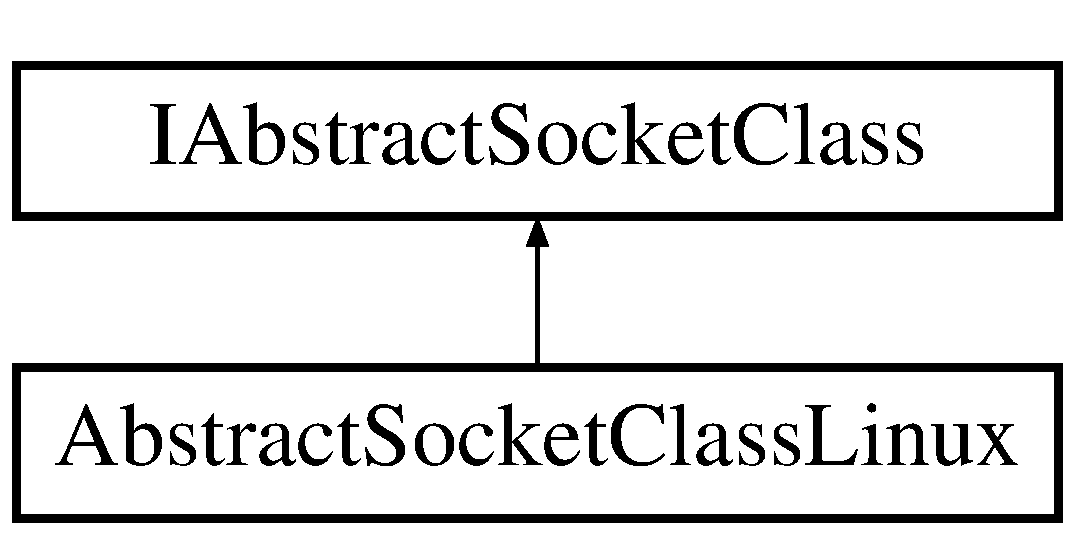
\includegraphics[height=2.000000cm]{class_abstract_socket_class_linux}
\end{center}
\end{figure}
\subsection*{Public Member Functions}
\begin{DoxyCompactItemize}
\item 
\hypertarget{class_abstract_socket_class_linux_aad61b4acfa08c8001d5b9d82d18a04a4}{
{\bfseries AbstractSocketClassLinux} (unsigned int port, std::string DocumentRoot, std::string XmlPath)}
\label{class_abstract_socket_class_linux_aad61b4acfa08c8001d5b9d82d18a04a4}

\item 
\hypertarget{class_abstract_socket_class_linux_abdad7a97f3a4671b2ea56bf02f8e28cb}{
virtual int {\bfseries StartServer} ()}
\label{class_abstract_socket_class_linux_abdad7a97f3a4671b2ea56bf02f8e28cb}

\item 
\hypertarget{class_abstract_socket_class_linux_abd509af9a70b82794050e1b70ad09e20}{
virtual int {\bfseries StopServer} ()}
\label{class_abstract_socket_class_linux_abd509af9a70b82794050e1b70ad09e20}

\end{DoxyCompactItemize}


The documentation for this class was generated from the following files:\begin{DoxyCompactItemize}
\item 
ZiaServer/abstractsocketclasslinux.h\item 
ZiaServer/abstractsocketclasslinux.cpp\end{DoxyCompactItemize}

\hypertarget{class_abstract_socket_class_windows}{
\section{AbstractSocketClassWindows Class Reference}
\label{class_abstract_socket_class_windows}\index{AbstractSocketClassWindows@{AbstractSocketClassWindows}}
}
Inheritance diagram for AbstractSocketClassWindows:\begin{figure}[H]
\begin{center}
\leavevmode
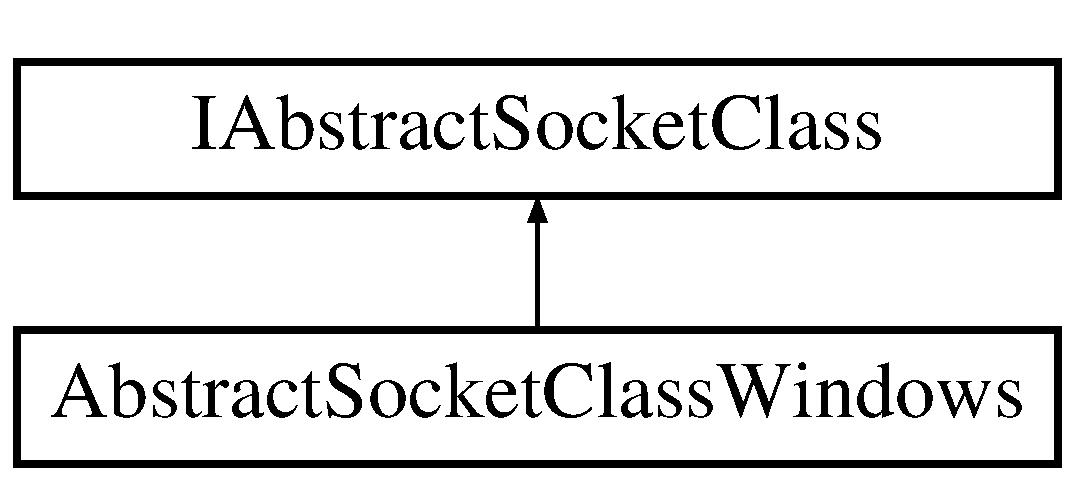
\includegraphics[height=2.000000cm]{class_abstract_socket_class_windows}
\end{center}
\end{figure}
\subsection*{Public Member Functions}
\begin{DoxyCompactItemize}
\item 
\hypertarget{class_abstract_socket_class_windows_ad4f8b40d469b68dc710d0cf007803ec0}{
{\bfseries AbstractSocketClassWindows} (unsigned int port, std::string DocumentRoot, std::string XmlPath)}
\label{class_abstract_socket_class_windows_ad4f8b40d469b68dc710d0cf007803ec0}

\item 
\hypertarget{class_abstract_socket_class_windows_a59e30f87c91be4536adb4f51f08086c6}{
virtual int {\bfseries StartServer} ()}
\label{class_abstract_socket_class_windows_a59e30f87c91be4536adb4f51f08086c6}

\item 
\hypertarget{class_abstract_socket_class_windows_afafe9b05475ecf89dad99d8565b324fa}{
virtual int {\bfseries StopServer} ()}
\label{class_abstract_socket_class_windows_afafe9b05475ecf89dad99d8565b324fa}

\end{DoxyCompactItemize}


The documentation for this class was generated from the following files:\begin{DoxyCompactItemize}
\item 
ZiaServer/abstractsocketclasswindows.h\item 
ZiaServer/abstractsocketclassWindows.cpp\end{DoxyCompactItemize}

\hypertarget{struct_client_data}{
\section{ClientData Struct Reference}
\label{struct_client_data}\index{ClientData@{ClientData}}
}
\subsection*{Public Attributes}
\begin{DoxyCompactItemize}
\item 
\hypertarget{struct_client_data_a23b2f90a351ac93b2a3ee559aadc8b9f}{
int {\bfseries socket}}
\label{struct_client_data_a23b2f90a351ac93b2a3ee559aadc8b9f}

\item 
\hypertarget{struct_client_data_a469182d11f1c996e63b47a52ebf04de4}{
int {\bfseries port}}
\label{struct_client_data_a469182d11f1c996e63b47a52ebf04de4}

\item 
\hypertarget{struct_client_data_a918292163843f45e026a74f20e11be35}{
std::string {\bfseries ip}}
\label{struct_client_data_a918292163843f45e026a74f20e11be35}

\item 
\hypertarget{struct_client_data_ac0943d293209a738bcbe836cd64087b7}{
std::string {\bfseries DocumentRoot}}
\label{struct_client_data_ac0943d293209a738bcbe836cd64087b7}

\item 
\hypertarget{struct_client_data_a6bfed9f1c1bcd8931ccc98c5bfc33c53}{
std::string {\bfseries XmlPath}}
\label{struct_client_data_a6bfed9f1c1bcd8931ccc98c5bfc33c53}

\end{DoxyCompactItemize}


The documentation for this struct was generated from the following file:\begin{DoxyCompactItemize}
\item 
ZiaServer/AbstractSocketClass.h\end{DoxyCompactItemize}

\hypertarget{class_command_panel_c_l_i}{
\section{CommandPanelCLI Class Reference}
\label{class_command_panel_c_l_i}\index{CommandPanelCLI@{CommandPanelCLI}}
}
Inheritance diagram for CommandPanelCLI:\begin{figure}[H]
\begin{center}
\leavevmode
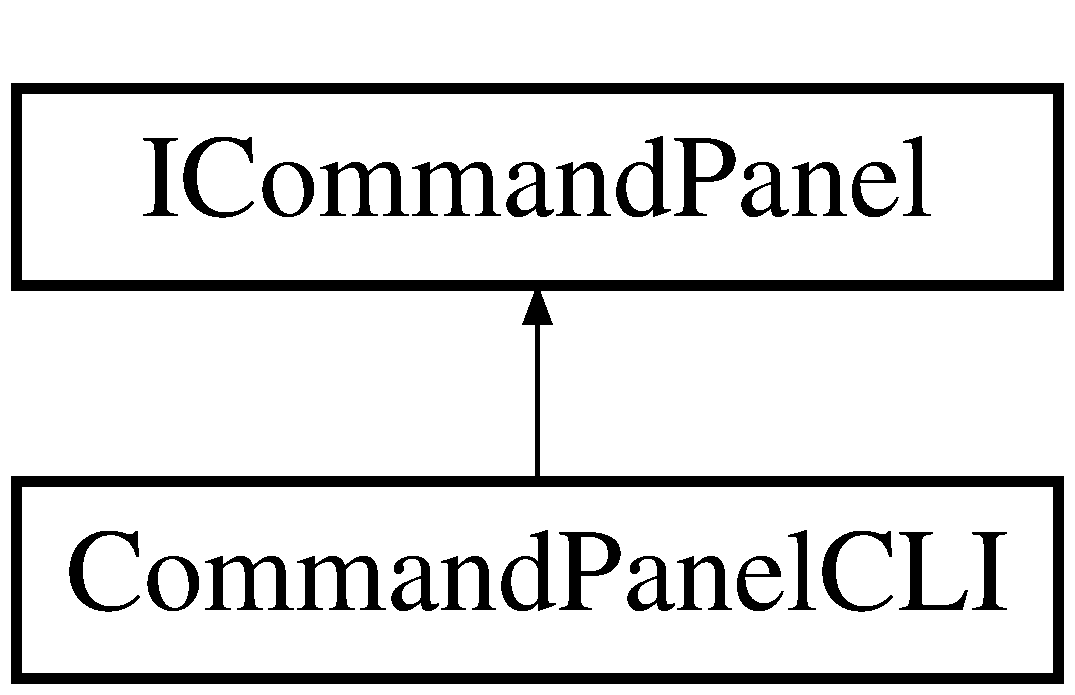
\includegraphics[height=2.000000cm]{class_command_panel_c_l_i}
\end{center}
\end{figure}
\subsection*{Public Member Functions}
\begin{DoxyCompactItemize}
\item 
\hypertarget{class_command_panel_c_l_i_a6b3ca62ce3e205a2db629a8b148eb497}{
{\bfseries CommandPanelCLI} (int argc, char $\ast$argv\mbox{[}$\,$\mbox{]})}
\label{class_command_panel_c_l_i_a6b3ca62ce3e205a2db629a8b148eb497}

\item 
\hypertarget{class_command_panel_c_l_i_a23691d223437b8eff265b7e9833e6ebf}{
virtual int {\bfseries start} ()}
\label{class_command_panel_c_l_i_a23691d223437b8eff265b7e9833e6ebf}

\item 
\hypertarget{class_command_panel_c_l_i_ac16eb64c8081ca93f946f4fa27c472b4}{
virtual int {\bfseries stop} ()}
\label{class_command_panel_c_l_i_ac16eb64c8081ca93f946f4fa27c472b4}

\item 
\hypertarget{class_command_panel_c_l_i_a0cb7d4a39d25b142b066549c1f58ee2d}{
virtual int {\bfseries restart} ()}
\label{class_command_panel_c_l_i_a0cb7d4a39d25b142b066549c1f58ee2d}

\item 
\hypertarget{class_command_panel_c_l_i_aad32b43d5753c717fad2ea0e55463ec5}{
void {\bfseries ShellStopFunction} (char $\ast$buf)}
\label{class_command_panel_c_l_i_aad32b43d5753c717fad2ea0e55463ec5}

\end{DoxyCompactItemize}
\subsection*{Static Public Member Functions}
\begin{DoxyCompactItemize}
\item 
\hypertarget{class_command_panel_c_l_i_aa86e91479f29c6d6ad1a7073d8589e5a}{
static void {\bfseries printState} (int code)}
\label{class_command_panel_c_l_i_aa86e91479f29c6d6ad1a7073d8589e5a}

\end{DoxyCompactItemize}


The documentation for this class was generated from the following files:\begin{DoxyCompactItemize}
\item 
ZiaServer/commandpanelcli.h\item 
ZiaServer/commandpanelcli.cpp\end{DoxyCompactItemize}

\hypertarget{struct_c_panel_data}{
\section{CPanelData Struct Reference}
\label{struct_c_panel_data}\index{CPanelData@{CPanelData}}
}
\subsection*{Public Attributes}
\begin{DoxyCompactItemize}
\item 
\hypertarget{struct_c_panel_data_a6d94c2ba25e461a028fa438ed9b73641}{
\hyperlink{class_abstract_socket_class_windows}{AbstractSocketClassWindows} $\ast$ {\bfseries network}}
\label{struct_c_panel_data_a6d94c2ba25e461a028fa438ed9b73641}

\item 
\hypertarget{struct_c_panel_data_a6768b2edcb478e0f15f20cf7d5e73943}{
int $\ast$ {\bfseries CPanelErrno}}
\label{struct_c_panel_data_a6768b2edcb478e0f15f20cf7d5e73943}

\item 
\hypertarget{struct_c_panel_data_ae94d23f4794c1da621be7faf37022327}{
pthread\_\-t $\ast$ {\bfseries thread}}
\label{struct_c_panel_data_ae94d23f4794c1da621be7faf37022327}

\end{DoxyCompactItemize}


The documentation for this struct was generated from the following file:\begin{DoxyCompactItemize}
\item 
ZiaServer/ICommandPanel.h\end{DoxyCompactItemize}

\hypertarget{struct_c_panel_state}{
\section{CPanelState Struct Reference}
\label{struct_c_panel_state}\index{CPanelState@{CPanelState}}
}
\subsection*{Public Attributes}
\begin{DoxyCompactItemize}
\item 
\hypertarget{struct_c_panel_state_afe3d637639b6c42c0121d9cc142df329}{
bool $\ast$ {\bfseries state}}
\label{struct_c_panel_state_afe3d637639b6c42c0121d9cc142df329}

\item 
\hypertarget{struct_c_panel_state_acdf201f4a8a760eb92c7159fb7d3207f}{
QLabel $\ast$ {\bfseries StateImage}}
\label{struct_c_panel_state_acdf201f4a8a760eb92c7159fb7d3207f}

\item 
\hypertarget{struct_c_panel_state_ab0728c745859db235ac020cc5b95727a}{
int $\ast$ {\bfseries CPanelErrno}}
\label{struct_c_panel_state_ab0728c745859db235ac020cc5b95727a}

\item 
\hypertarget{struct_c_panel_state_a6f96cbe80459edf7b467b9b3b310289a}{
pthread\_\-t $\ast$ {\bfseries thread}}
\label{struct_c_panel_state_a6f96cbe80459edf7b467b9b3b310289a}

\item 
\hypertarget{struct_c_panel_state_a432d9edf67fd7888c5a78e54d217d437}{
\hyperlink{classgui}{gui} $\ast$ {\bfseries guiPointer}}
\label{struct_c_panel_state_a432d9edf67fd7888c5a78e54d217d437}

\end{DoxyCompactItemize}


The documentation for this struct was generated from the following file:\begin{DoxyCompactItemize}
\item 
ZiaServer/Gui/gui.h\end{DoxyCompactItemize}

\hypertarget{class_ecriture_dom}{
\section{EcritureDom Class Reference}
\label{class_ecriture_dom}\index{EcritureDom@{EcritureDom}}
}
\subsection*{Public Slots}
\begin{DoxyCompactItemize}
\item 
\hypertarget{class_ecriture_dom_a87f7c942f08de38d8f00850553d658e7}{
void {\bfseries maj\_\-fichier} (\hyperlink{class_zia}{Zia} \&proj)}
\label{class_ecriture_dom_a87f7c942f08de38d8f00850553d658e7}

\end{DoxyCompactItemize}


The documentation for this class was generated from the following files:\begin{DoxyCompactItemize}
\item 
ZiaServer/xml/SaveXML.h\item 
ZiaServer/xml/SaveXML.cpp\end{DoxyCompactItemize}

\hypertarget{structfile}{
\section{file Struct Reference}
\label{structfile}\index{file@{file}}
}
\subsection*{Public Attributes}
\begin{DoxyCompactItemize}
\item 
\hypertarget{structfile_a4714478b17f2b5a3a8bc869a259f27f8}{
std::string {\bfseries filename}}
\label{structfile_a4714478b17f2b5a3a8bc869a259f27f8}

\item 
\hypertarget{structfile_ac5e7f0443a85241e529105097fe17924}{
std::string {\bfseries filepath}}
\label{structfile_ac5e7f0443a85241e529105097fe17924}

\item 
\hypertarget{structfile_a61d9c58c5cfb4e0ae94c57686509bb37}{
std::string {\bfseries ext}}
\label{structfile_a61d9c58c5cfb4e0ae94c57686509bb37}

\end{DoxyCompactItemize}


The documentation for this struct was generated from the following file:\begin{DoxyCompactItemize}
\item 
ZiaServer/zfile.h\end{DoxyCompactItemize}

\hypertarget{structfolder}{
\section{folder Struct Reference}
\label{structfolder}\index{folder@{folder}}
}
\subsection*{Public Attributes}
\begin{DoxyCompactItemize}
\item 
\hypertarget{structfolder_a3e484208c282ad2552bd84ea4ca79242}{
std::string {\bfseries filename}}
\label{structfolder_a3e484208c282ad2552bd84ea4ca79242}

\item 
\hypertarget{structfolder_a8f3d16f6b6f792acf0fd95fc0d48875c}{
std::string {\bfseries filepath}}
\label{structfolder_a8f3d16f6b6f792acf0fd95fc0d48875c}

\item 
\hypertarget{structfolder_a6ebf50c67fb55c0f7f3a4469ace26768}{
std::string {\bfseries ext}}
\label{structfolder_a6ebf50c67fb55c0f7f3a4469ace26768}

\end{DoxyCompactItemize}


The documentation for this struct was generated from the following file:\begin{DoxyCompactItemize}
\item 
ZiaServer/zfile.h\end{DoxyCompactItemize}

\hypertarget{classgui}{
\section{gui Class Reference}
\label{classgui}\index{gui@{gui}}
}
Inheritance diagram for gui:\begin{figure}[H]
\begin{center}
\leavevmode
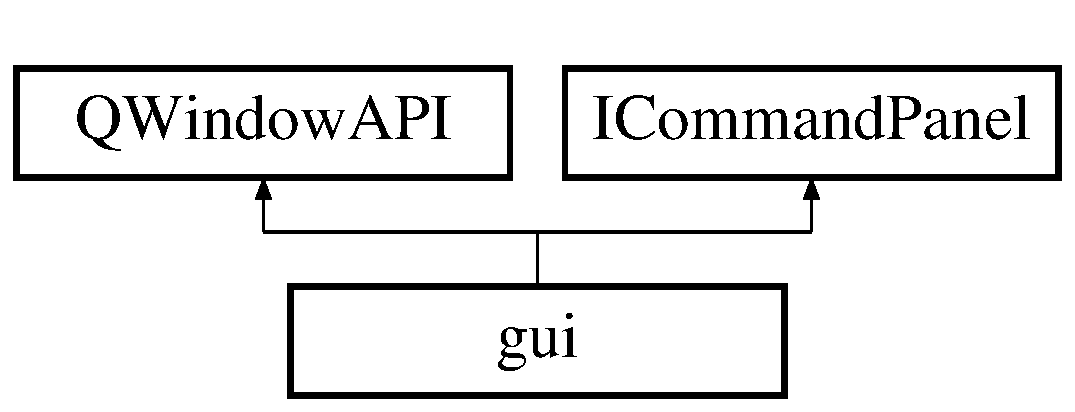
\includegraphics[height=2.000000cm]{classgui}
\end{center}
\end{figure}
\subsection*{Public Slots}
\begin{DoxyCompactItemize}
\item 
\hypertarget{classgui_aada4b3c2985867563163060b0ea7790a}{
void {\bfseries ModulesWindow} ()}
\label{classgui_aada4b3c2985867563163060b0ea7790a}

\item 
\hypertarget{classgui_a635d4673ab60e67174d1070188d45cde}{
int {\bfseries start} ()}
\label{classgui_a635d4673ab60e67174d1070188d45cde}

\item 
\hypertarget{classgui_a25ea2b9bce229c4955b6cf426f865ff4}{
int {\bfseries stop} ()}
\label{classgui_a25ea2b9bce229c4955b6cf426f865ff4}

\item 
\hypertarget{classgui_aa714d6bf36da2b9d2410aa556f6cf7c0}{
int {\bfseries restart} ()}
\label{classgui_aa714d6bf36da2b9d2410aa556f6cf7c0}

\item 
\hypertarget{classgui_a70aa201aa78f95ff25d15ce177a46b88}{
void {\bfseries PortInputChange} (QString data)}
\label{classgui_a70aa201aa78f95ff25d15ce177a46b88}

\item 
\hypertarget{classgui_a6a0822f02ed0c3cd48b6a59349e4827c}{
void {\bfseries DocumentRootInputChange} (QString data)}
\label{classgui_a6a0822f02ed0c3cd48b6a59349e4827c}

\item 
\hypertarget{classgui_a1ab76a511d9af11dcf4857233fcd2d39}{
void {\bfseries DocumentRootBrowse} ()}
\label{classgui_a1ab76a511d9af11dcf4857233fcd2d39}

\item 
\hypertarget{classgui_a2777443c9f0136f570e1f31f45443782}{
void {\bfseries HandleDocumentRoot} (QString \hyperlink{structfolder}{folder})}
\label{classgui_a2777443c9f0136f570e1f31f45443782}

\item 
\hypertarget{classgui_ab985f43855c8bb7a20f2028882ebc263}{
void {\bfseries slotTrayActivated} (QSystemTrayIcon::ActivationReason reason)}
\label{classgui_ab985f43855c8bb7a20f2028882ebc263}

\item 
\hypertarget{classgui_a072be3b09b6fccdbe12cf2d335277b65}{
bool {\bfseries tray} ()}
\label{classgui_a072be3b09b6fccdbe12cf2d335277b65}

\end{DoxyCompactItemize}
\subsection*{Public Member Functions}
\begin{DoxyCompactItemize}
\item 
\hypertarget{classgui_a4039d74471f0f05e7d64a1459d7c4e41}{
{\bfseries gui} (const char $\ast$name, int width, int height, bool frame, QString logo, QString filename)}
\label{classgui_a4039d74471f0f05e7d64a1459d7c4e41}

\end{DoxyCompactItemize}
\subsection*{Static Public Member Functions}
\begin{DoxyCompactItemize}
\item 
\hypertarget{classgui_a7d216373d047ee4e0546ce0c63d4b2bf}{
static void {\bfseries printState} (int code)}
\label{classgui_a7d216373d047ee4e0546ce0c63d4b2bf}

\end{DoxyCompactItemize}


The documentation for this class was generated from the following files:\begin{DoxyCompactItemize}
\item 
ZiaServer/Gui/gui.h\item 
ZiaServer/Gui/gui.cpp\end{DoxyCompactItemize}

\hypertarget{class_i_abstract_socket_class}{
\section{IAbstractSocketClass Class Reference}
\label{class_i_abstract_socket_class}\index{IAbstractSocketClass@{IAbstractSocketClass}}
}
Inheritance diagram for IAbstractSocketClass:\begin{figure}[H]
\begin{center}
\leavevmode
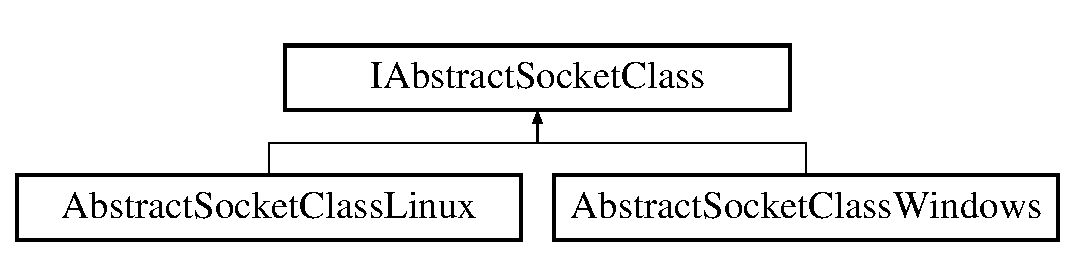
\includegraphics[height=2.000000cm]{class_i_abstract_socket_class}
\end{center}
\end{figure}


The documentation for this class was generated from the following file:\begin{DoxyCompactItemize}
\item 
ZiaServer/AbstractSocketClass.h\end{DoxyCompactItemize}

\hypertarget{class_i_command_panel}{
\section{ICommandPanel Class Reference}
\label{class_i_command_panel}\index{ICommandPanel@{ICommandPanel}}
}
Inheritance diagram for ICommandPanel:\begin{figure}[H]
\begin{center}
\leavevmode
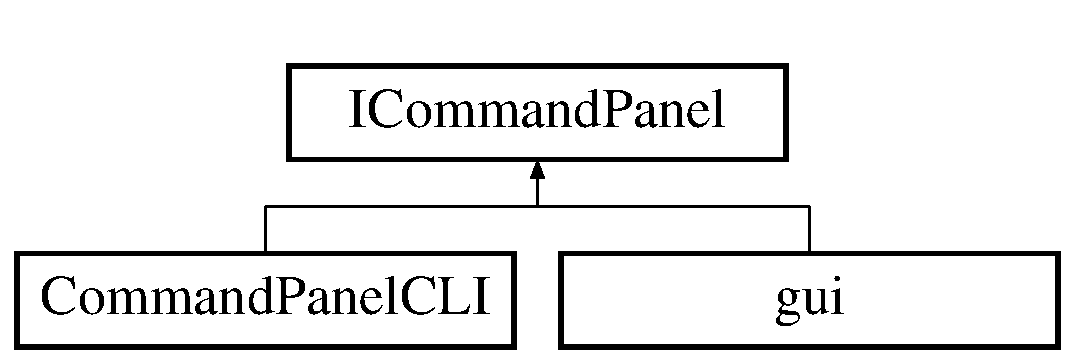
\includegraphics[height=2.000000cm]{class_i_command_panel}
\end{center}
\end{figure}
\subsection*{Public Member Functions}
\begin{DoxyCompactItemize}
\item 
\hypertarget{class_i_command_panel_a740f6e219fadf8eb42bca24fb5d2facc}{
virtual int {\bfseries start} ()=0}
\label{class_i_command_panel_a740f6e219fadf8eb42bca24fb5d2facc}

\item 
\hypertarget{class_i_command_panel_a3655a8d2d748f369a6a3691428992ddb}{
virtual int {\bfseries stop} ()=0}
\label{class_i_command_panel_a3655a8d2d748f369a6a3691428992ddb}

\item 
\hypertarget{class_i_command_panel_ab186158f2cdf60fe116df3d4f6eec399}{
virtual int {\bfseries restart} ()=0}
\label{class_i_command_panel_ab186158f2cdf60fe116df3d4f6eec399}

\item 
\hypertarget{class_i_command_panel_a4db30265210e012ccadc80311270c7bb}{
virtual bool {\bfseries getState} ()}
\label{class_i_command_panel_a4db30265210e012ccadc80311270c7bb}

\end{DoxyCompactItemize}
\subsection*{Protected Attributes}
\begin{DoxyCompactItemize}
\item 
\hypertarget{class_i_command_panel_a4f6ea46e98133e4fae91117abeec5ef6}{
bool {\bfseries state}}
\label{class_i_command_panel_a4f6ea46e98133e4fae91117abeec5ef6}

\item 
\hypertarget{class_i_command_panel_af1c73d5075c578cca49bcc62d7c438b4}{
int {\bfseries port}}
\label{class_i_command_panel_af1c73d5075c578cca49bcc62d7c438b4}

\item 
\hypertarget{class_i_command_panel_adab357fffc6bed0d5cd02b65b05206f6}{
int {\bfseries CPanelErrno}}
\label{class_i_command_panel_adab357fffc6bed0d5cd02b65b05206f6}

\item 
\hypertarget{class_i_command_panel_afe3ea1eb7fb365dfaa843edf729a525b}{
std::string {\bfseries DocumentRoot}}
\label{class_i_command_panel_afe3ea1eb7fb365dfaa843edf729a525b}

\item 
\hypertarget{class_i_command_panel_a929066b973dcaaff260127bb7b25ae95}{
std::string {\bfseries XmlPath}}
\label{class_i_command_panel_a929066b973dcaaff260127bb7b25ae95}

\end{DoxyCompactItemize}


The documentation for this class was generated from the following file:\begin{DoxyCompactItemize}
\item 
ZiaServer/ICommandPanel.h\end{DoxyCompactItemize}

\hypertarget{class_lecture___d_o_m}{
\section{Lecture\_\-DOM Class Reference}
\label{class_lecture___d_o_m}\index{Lecture\_\-DOM@{Lecture\_\-DOM}}
}
\subsection*{Public Member Functions}
\begin{DoxyCompactItemize}
\item 
\hypertarget{class_lecture___d_o_m_a384f1b6e1813a352cfc2bcb06714decd}{
void {\bfseries lire} (\hyperlink{class_zia}{Zia} \&proj)}
\label{class_lecture___d_o_m_a384f1b6e1813a352cfc2bcb06714decd}

\end{DoxyCompactItemize}
\subsection*{Static Public Member Functions}
\begin{DoxyCompactItemize}
\item 
\hypertarget{class_lecture___d_o_m_a0ab8e2bbaf8acdf19fc6d04984af1027}{
static bool {\bfseries ValidityFile} ()}
\label{class_lecture___d_o_m_a0ab8e2bbaf8acdf19fc6d04984af1027}

\end{DoxyCompactItemize}


The documentation for this class was generated from the following files:\begin{DoxyCompactItemize}
\item 
ZiaServer/xml/Lecture.h\item 
ZiaServer/xml/Lecture.cpp\end{DoxyCompactItemize}

\hypertarget{structmime}{
\section{mime Struct Reference}
\label{structmime}\index{mime@{mime}}
}
\subsection*{Public Attributes}
\begin{DoxyCompactItemize}
\item 
\hypertarget{structmime_a2008e2ca1f2d0f09c41f83b37cef9754}{
std::string {\bfseries name}}
\label{structmime_a2008e2ca1f2d0f09c41f83b37cef9754}

\item 
\hypertarget{structmime_a87554d0aba281e598a0082abcc61d889}{
std::string {\bfseries type}}
\label{structmime_a87554d0aba281e598a0082abcc61d889}

\end{DoxyCompactItemize}


The documentation for this struct was generated from the following file:\begin{DoxyCompactItemize}
\item 
ZiaServer/zfile.h\end{DoxyCompactItemize}

\hypertarget{class_module}{
\section{Module Class Reference}
\label{class_module}\index{Module@{Module}}
}
\subsection*{Public Member Functions}
\begin{DoxyCompactItemize}
\item 
\hypertarget{class_module_a09034ae475aca93c53de6f68d0b5fdf4}{
void {\bfseries addType} (QString)}
\label{class_module_a09034ae475aca93c53de6f68d0b5fdf4}

\item 
\hypertarget{class_module_a5ac684440ce769072d08d43b7e1151e6}{
void {\bfseries setName} (QString)}
\label{class_module_a5ac684440ce769072d08d43b7e1151e6}

\item 
\hypertarget{class_module_a7146d5328a353dd742c88e30805e881e}{
void {\bfseries setPath} (QString)}
\label{class_module_a7146d5328a353dd742c88e30805e881e}

\item 
\hypertarget{class_module_a5bbce6b4f2b695d3e114b97ad0ca4f18}{
QString {\bfseries getName} () const }
\label{class_module_a5bbce6b4f2b695d3e114b97ad0ca4f18}

\item 
\hypertarget{class_module_a4e2c6e41fa2f788f6af316beb9476aa3}{
QString {\bfseries getPath} () const }
\label{class_module_a4e2c6e41fa2f788f6af316beb9476aa3}

\item 
\hypertarget{class_module_abbfeaf9d7d7e35ade6dfad50cc043e34}{
{\bfseries Module} (const \hyperlink{class_module}{Module} \&)}
\label{class_module_abbfeaf9d7d7e35ade6dfad50cc043e34}

\item 
\hypertarget{class_module_a23b9518198af877726208c1d6312d4ab}{
\hyperlink{class_module}{Module} \& {\bfseries operator=} (const \hyperlink{class_module}{Module} \&)}
\label{class_module_a23b9518198af877726208c1d6312d4ab}

\end{DoxyCompactItemize}
\subsection*{Public Attributes}
\begin{DoxyCompactItemize}
\item 
\hypertarget{class_module_a509034a09559607535f6372a7552ae89}{
QList$<$ QString $>$ {\bfseries type}}
\label{class_module_a509034a09559607535f6372a7552ae89}

\end{DoxyCompactItemize}


The documentation for this class was generated from the following files:\begin{DoxyCompactItemize}
\item 
ZiaServer/xml/module.h\item 
ZiaServer/xml/module.cpp\end{DoxyCompactItemize}

\hypertarget{class_modules_window_class}{
\section{ModulesWindowClass Class Reference}
\label{class_modules_window_class}\index{ModulesWindowClass@{ModulesWindowClass}}
}
Inheritance diagram for ModulesWindowClass:\begin{figure}[H]
\begin{center}
\leavevmode
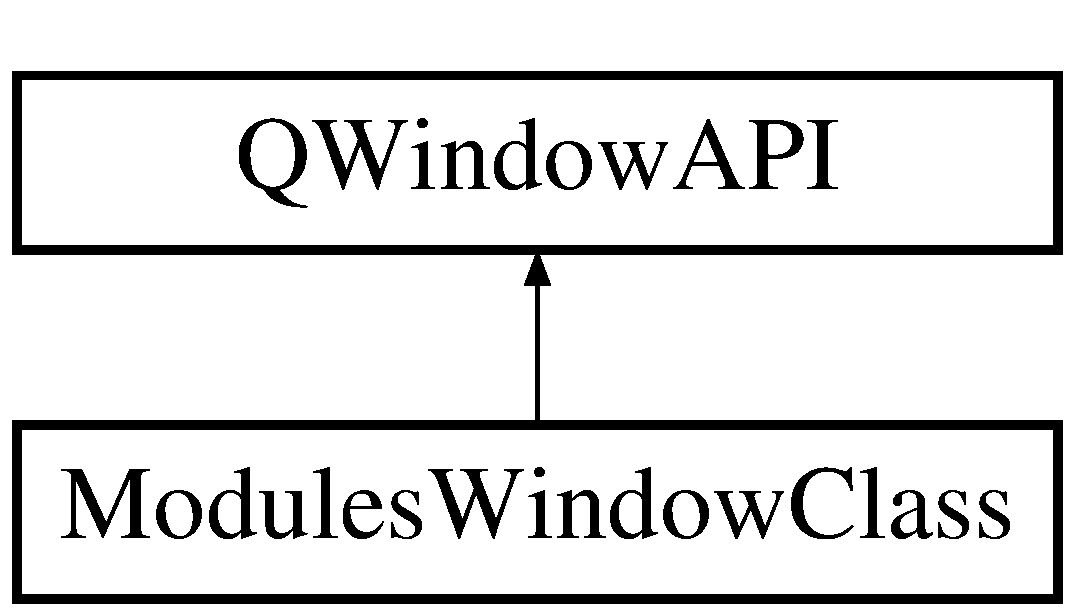
\includegraphics[height=2.000000cm]{class_modules_window_class}
\end{center}
\end{figure}
\subsection*{Public Slots}
\begin{DoxyCompactItemize}
\item 
\hypertarget{class_modules_window_class_a407ecce7f578aa4b183093779517ecd0}{
void {\bfseries SaveIndex} (QModelIndex index)}
\label{class_modules_window_class_a407ecce7f578aa4b183093779517ecd0}

\item 
\hypertarget{class_modules_window_class_a8617df7392acea1c11e1124e27621290}{
void {\bfseries AddModule} ()}
\label{class_modules_window_class_a8617df7392acea1c11e1124e27621290}

\item 
\hypertarget{class_modules_window_class_a21e1219a34cd23bb3932d6863aec17b0}{
void {\bfseries DeleteModule} ()}
\label{class_modules_window_class_a21e1219a34cd23bb3932d6863aec17b0}

\item 
\hypertarget{class_modules_window_class_ae23d0ad58531e4175e90c00d150803cf}{
void {\bfseries HandleFile} (QString \hyperlink{structfile}{file})}
\label{class_modules_window_class_ae23d0ad58531e4175e90c00d150803cf}

\end{DoxyCompactItemize}
\subsection*{Public Member Functions}
\begin{DoxyCompactItemize}
\item 
\hypertarget{class_modules_window_class_a5f2d43af6761e0ab838bd023f847a009}{
{\bfseries ModulesWindowClass} (const char $\ast$name, int width, int height, bool frame, QString logo, QString filename)}
\label{class_modules_window_class_a5f2d43af6761e0ab838bd023f847a009}

\item 
\hypertarget{class_modules_window_class_ae6670c8b282f104cec39a18050274e8c}{
\hyperlink{class_modules_window_class}{ModulesWindowClass} $\ast$ {\bfseries Instance} ()}
\label{class_modules_window_class_ae6670c8b282f104cec39a18050274e8c}

\end{DoxyCompactItemize}


The documentation for this class was generated from the following files:\begin{DoxyCompactItemize}
\item 
ZiaServer/Gui/moduleswindow.h\item 
ZiaServer/Gui/moduleswindow.cpp\end{DoxyCompactItemize}

\hypertarget{class_q_window_a_p_i}{
\section{QWindowAPI Class Reference}
\label{class_q_window_a_p_i}\index{QWindowAPI@{QWindowAPI}}
}
Inheritance diagram for QWindowAPI:\begin{figure}[H]
\begin{center}
\leavevmode
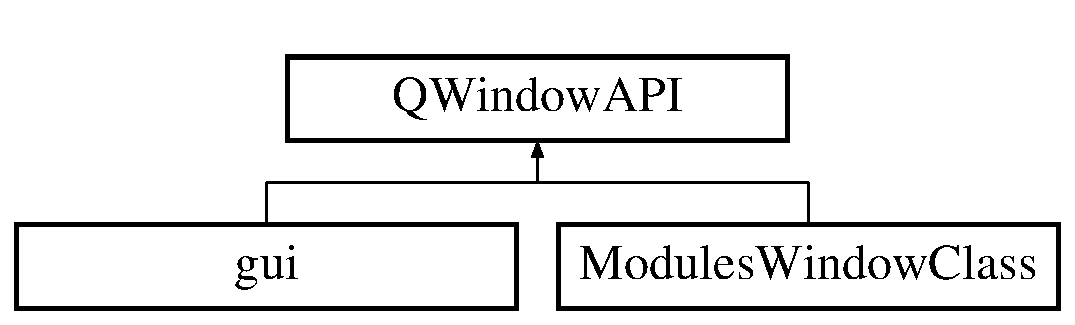
\includegraphics[height=2.000000cm]{class_q_window_a_p_i}
\end{center}
\end{figure}
\subsection*{Public Member Functions}
\begin{DoxyCompactItemize}
\item 
\hypertarget{class_q_window_a_p_i_ae8211c69c07c3831218c6098ecc6aaf5}{
{\bfseries QWindowAPI} (const char $\ast$name, int width, int height, bool frame, QString logo, QString filename)}
\label{class_q_window_a_p_i_ae8211c69c07c3831218c6098ecc6aaf5}

\end{DoxyCompactItemize}
\subsection*{Protected Member Functions}
\begin{DoxyCompactItemize}
\item 
\hypertarget{class_q_window_a_p_i_a178d3e0dbd8873879d3f08f97ee0a772}{
virtual QPushButton $\ast$ {\bfseries CreateButton} (QWidget $\ast$widget, const char $\ast$name, int height, int width, int pos\_\-x, int pos\_\-y, const QString stylesheet=\char`\"{}\char`\"{})}
\label{class_q_window_a_p_i_a178d3e0dbd8873879d3f08f97ee0a772}

\item 
\hypertarget{class_q_window_a_p_i_a439a14ace5436d4c2ed7627fc4e972ec}{
virtual QListView $\ast$ {\bfseries CreateList} (QWidget $\ast$widget, int height, int width, int pos\_\-x, int pos\_\-y)=0}
\label{class_q_window_a_p_i_a439a14ace5436d4c2ed7627fc4e972ec}

\item 
\hypertarget{class_q_window_a_p_i_a2d2c92d10ce54ea32ceb8928b2733572}{
virtual QLineEdit $\ast$ {\bfseries CreateInputBox} (QWidget $\ast$widget, int height, int width, int pos\_\-x, int pos\_\-y, int mode)}
\label{class_q_window_a_p_i_a2d2c92d10ce54ea32ceb8928b2733572}

\item 
\hypertarget{class_q_window_a_p_i_ac637916d5e5e2b72d3549afc8ed607a1}{
virtual QLabel $\ast$ {\bfseries CreateLink} (QWidget $\ast$widget, QString text, int pos\_\-x, int pos\_\-y, const QString \hyperlink{classtype}{type}=NULL)}
\label{class_q_window_a_p_i_ac637916d5e5e2b72d3549afc8ed607a1}

\item 
\hypertarget{class_q_window_a_p_i_ad3c7dfefa0a822e4ae4f4223704981d9}{
virtual QLabel $\ast$ {\bfseries CreateText} (QWidget $\ast$widget, QString text, int width, int height, int pos\_\-x, int pos\_\-y)}
\label{class_q_window_a_p_i_ad3c7dfefa0a822e4ae4f4223704981d9}

\item 
\hypertarget{class_q_window_a_p_i_a8bff56b9568061b2c004d6e8b3c5dcaa}{
virtual QLabel $\ast$ {\bfseries CreateImage} (QWidget $\ast$widget, const QString filename, int height, int width, int pos\_\-x, int pos\_\-y)}
\label{class_q_window_a_p_i_a8bff56b9568061b2c004d6e8b3c5dcaa}

\item 
\hypertarget{class_q_window_a_p_i_aab8041714388aabab71843ca09fac646}{
virtual QPushButton $\ast$ {\bfseries CreateClickableImage} (QWidget $\ast$widget, const QString filename, int height, int width, int pos\_\-x, int pos\_\-y)}
\label{class_q_window_a_p_i_aab8041714388aabab71843ca09fac646}

\item 
\hypertarget{class_q_window_a_p_i_a9b0dee3c3c4c75b5a48c6a8d7e78b269}{
virtual void {\bfseries mousePressEvent} (QMouseEvent $\ast$event)}
\label{class_q_window_a_p_i_a9b0dee3c3c4c75b5a48c6a8d7e78b269}

\item 
\hypertarget{class_q_window_a_p_i_a158948ba8f512fa23f88ac10c97f9e06}{
virtual void {\bfseries mouseReleaseEvent} (QMouseEvent $\ast$event)}
\label{class_q_window_a_p_i_a158948ba8f512fa23f88ac10c97f9e06}

\item 
\hypertarget{class_q_window_a_p_i_a3bb8dbfeb69f26147e5990f66151692e}{
virtual void {\bfseries mouseMoveEvent} (QMouseEvent $\ast$event)}
\label{class_q_window_a_p_i_a3bb8dbfeb69f26147e5990f66151692e}

\end{DoxyCompactItemize}
\subsection*{Protected Attributes}
\begin{DoxyCompactItemize}
\item 
\hypertarget{class_q_window_a_p_i_ac510ee00f76bc4721d58f12f8a53d8f3}{
QStandardItemModel $\ast$ {\bfseries iStandardModel}}
\label{class_q_window_a_p_i_ac510ee00f76bc4721d58f12f8a53d8f3}

\item 
\hypertarget{class_q_window_a_p_i_a30c1d4ae0e9d24418026e0a553290fbb}{
QPoint {\bfseries m\_\-Diff}}
\label{class_q_window_a_p_i_a30c1d4ae0e9d24418026e0a553290fbb}

\end{DoxyCompactItemize}


The documentation for this class was generated from the following files:\begin{DoxyCompactItemize}
\item 
ZiaServer/Gui/qwindowapi.h\item 
ZiaServer/Gui/qwindow.cpp\end{DoxyCompactItemize}

\hypertarget{class_reponse}{
\section{Reponse Class Reference}
\label{class_reponse}\index{Reponse@{Reponse}}
}
\subsection*{Public Member Functions}
\begin{DoxyCompactItemize}
\item 
\hypertarget{class_reponse_a64d485845bb40fe9d20f617b9b3ec9fd}{
{\bfseries Reponse} (std::string ServerName, std::string code, std::string httpVersion, std::string method, std::string contentType, int contentLength)}
\label{class_reponse_a64d485845bb40fe9d20f617b9b3ec9fd}

\item 
\hypertarget{class_reponse_a50c6e746b49d0edc7a7f9f180b76d69f}{
std::string {\bfseries getResponse} ()}
\label{class_reponse_a50c6e746b49d0edc7a7f9f180b76d69f}

\end{DoxyCompactItemize}


The documentation for this class was generated from the following files:\begin{DoxyCompactItemize}
\item 
ZiaServer/reponse.h\item 
ZiaServer/reponse.cpp\end{DoxyCompactItemize}

\hypertarget{classtype}{
\section{type Class Reference}
\label{classtype}\index{type@{type}}
}
\subsection*{Public Attributes}
\begin{DoxyCompactItemize}
\item 
\hypertarget{classtype_aca5a30fa5039605d18bded05c1db81c3}{
QString {\bfseries getType}}
\label{classtype_aca5a30fa5039605d18bded05c1db81c3}

\end{DoxyCompactItemize}


The documentation for this class was generated from the following file:\begin{DoxyCompactItemize}
\item 
ZiaServer/xml/type.h\end{DoxyCompactItemize}

\hypertarget{classz_file}{
\section{zFile Class Reference}
\label{classz_file}\index{zFile@{zFile}}
}
\subsection*{Public Member Functions}
\begin{DoxyCompactItemize}
\item 
\hypertarget{classz_file_adca0fbce0ce8549f020a003dfad2010e}{
{\bfseries zFile} (struct \hyperlink{structfolder}{folder} dossier, std::string DocumentRoot)}
\label{classz_file_adca0fbce0ce8549f020a003dfad2010e}

\item 
\hypertarget{classz_file_a959c8cf75930a623e0e1d48d97988d4b}{
{\bfseries zFile} (struct \hyperlink{structfile}{file} fichier, std::string DocumentRoot)}
\label{classz_file_a959c8cf75930a623e0e1d48d97988d4b}

\item 
\hypertarget{classz_file_a1031b8a37ed3fe9a3d90e36d1a327c9e}{
char $\ast$ {\bfseries getDocumentContent} ()}
\label{classz_file_a1031b8a37ed3fe9a3d90e36d1a327c9e}

\item 
\hypertarget{classz_file_a04b04ed0d4aede3f1fb70eb56a9197f7}{
std::string {\bfseries getFilePath} ()}
\label{classz_file_a04b04ed0d4aede3f1fb70eb56a9197f7}

\item 
\hypertarget{classz_file_af29fb6da0efb830c9c78af95d0231401}{
std::string {\bfseries getFileType} ()}
\label{classz_file_af29fb6da0efb830c9c78af95d0231401}

\item 
\hypertarget{classz_file_a79185017be3a17e64719741a6b760eda}{
std::string {\bfseries getFileExtension} ()}
\label{classz_file_a79185017be3a17e64719741a6b760eda}

\item 
\hypertarget{classz_file_a24032fa6a82b917c677aa2daa9caf989}{
int {\bfseries getDocumentLength} ()}
\label{classz_file_a24032fa6a82b917c677aa2daa9caf989}

\item 
\hypertarget{classz_file_a9522751785e090ee69dd71a19a0ffcbf}{
std::string {\bfseries getReturnCode} ()}
\label{classz_file_a9522751785e090ee69dd71a19a0ffcbf}

\item 
\hypertarget{classz_file_aa16dc434c176c74a36b4605f94d1009f}{
std::string {\bfseries getContentType} ()}
\label{classz_file_aa16dc434c176c74a36b4605f94d1009f}

\end{DoxyCompactItemize}


The documentation for this class was generated from the following files:\begin{DoxyCompactItemize}
\item 
ZiaServer/zfile.h\item 
ZiaServer/zfile.cpp\end{DoxyCompactItemize}

\hypertarget{class_zia}{
\section{Zia Class Reference}
\label{class_zia}\index{Zia@{Zia}}
}
\subsection*{Public Member Functions}
\begin{DoxyCompactItemize}
\item 
\hypertarget{class_zia_a89985973e8a61077be81bb8e52f1b561}{
void {\bfseries addModule} (QString, QString)}
\label{class_zia_a89985973e8a61077be81bb8e52f1b561}

\item 
\hypertarget{class_zia_a143184d0e0e5b230ce01b09c4b5f6604}{
void {\bfseries deleteModule} (QString)}
\label{class_zia_a143184d0e0e5b230ce01b09c4b5f6604}

\item 
\hypertarget{class_zia_add757b78a4d032477a4265680966358a}{
void {\bfseries setDocumentRoot} (QString)}
\label{class_zia_add757b78a4d032477a4265680966358a}

\item 
\hypertarget{class_zia_a92272b44eba95d3b4448decdacb53a65}{
void {\bfseries setPort} (int)}
\label{class_zia_a92272b44eba95d3b4448decdacb53a65}

\item 
\hypertarget{class_zia_aeff84536e61553bef4638c6c56bbef8c}{
void {\bfseries modifDocumentRoot} (QString)}
\label{class_zia_aeff84536e61553bef4638c6c56bbef8c}

\item 
\hypertarget{class_zia_a3009ed54a4cb32d4642a50461ac3a623}{
void {\bfseries modifPort} (int)}
\label{class_zia_a3009ed54a4cb32d4642a50461ac3a623}

\item 
\hypertarget{class_zia_ab7a46d3d492a5c91062f361240ce0c22}{
void {\bfseries addTypeByList} (QString \_\-module, QList$<$ QString $>$ \_\-type)}
\label{class_zia_ab7a46d3d492a5c91062f361240ce0c22}

\item 
\hypertarget{class_zia_a4bfe7ff815f67c92bf422eb22a67f034}{
void {\bfseries addTypeByOne} (QString \_\-module, QString \_\-type)}
\label{class_zia_a4bfe7ff815f67c92bf422eb22a67f034}

\item 
\hypertarget{class_zia_ac1dac746886d728cc9d5e7b7fe385745}{
void {\bfseries deleteType} (QString \_\-module, QString \_\-type)}
\label{class_zia_ac1dac746886d728cc9d5e7b7fe385745}

\item 
\hypertarget{class_zia_a08ee5e637cb97e9634b4a063aaea3627}{
void {\bfseries maj} ()}
\label{class_zia_a08ee5e637cb97e9634b4a063aaea3627}

\item 
\hypertarget{class_zia_a59e7342ba3a2727f812b0c847dca3bb4}{
int {\bfseries getPort} () const }
\label{class_zia_a59e7342ba3a2727f812b0c847dca3bb4}

\item 
\hypertarget{class_zia_a4922ff8a1f60db1460d4e901c9a2f576}{
QString {\bfseries getDocumentRoot} () const }
\label{class_zia_a4922ff8a1f60db1460d4e901c9a2f576}

\item 
\hypertarget{class_zia_a620d83f267fc11dba5aab9f90b175430}{
{\bfseries Zia} (const \hyperlink{class_zia}{Zia} \&)}
\label{class_zia_a620d83f267fc11dba5aab9f90b175430}

\item 
\hypertarget{class_zia_aa906c7502690cc20c41de8d57e9f2d62}{
\hyperlink{class_zia}{Zia} \& {\bfseries operator=} (const \hyperlink{class_zia}{Zia} \&)}
\label{class_zia_aa906c7502690cc20c41de8d57e9f2d62}

\end{DoxyCompactItemize}
\subsection*{Public Attributes}
\begin{DoxyCompactItemize}
\item 
\hypertarget{class_zia_ae720605acc85e38462fc027a901aacd6}{
QList$<$ \hyperlink{class_module}{Module} $>$ {\bfseries modules}}
\label{class_zia_ae720605acc85e38462fc027a901aacd6}

\item 
\hypertarget{class_zia_a908b0f461f5904d15cf89fd0d527d69b}{
QList$<$ QString $>$ {\bfseries default\_\-extensions}}
\label{class_zia_a908b0f461f5904d15cf89fd0d527d69b}

\item 
\hypertarget{class_zia_ae7d7142801576c6098205d9ebb90f2a5}{
QList$<$ QString $>$ {\bfseries forbidden\_\-path}}
\label{class_zia_ae7d7142801576c6098205d9ebb90f2a5}

\end{DoxyCompactItemize}


The documentation for this class was generated from the following files:\begin{DoxyCompactItemize}
\item 
ZiaServer/xml/zia.h\item 
ZiaServer/xml/zia.cpp\end{DoxyCompactItemize}

\printindex
\end{document}
